\documentclass[dvipsnames]{beamer}
\usepackage[utf8]{inputenc}
\usepackage{listings}
\usepackage{comment}
\usepackage{soul}
%\usepackage{ulem}
\usepackage{subfig}
\setul{}{1pt}
\usepackage[oldenum, olditem]{paralist}
%allow even smaller text
\newcommand\tinytiny{\fontsize{4pt}{3}\selectfont}

\makeatletter
\let\old@lstKV@SwitchCases\lstKV@SwitchCases
\def\lstKV@SwitchCases#1#2#3{}
\makeatother
\usepackage{lstlinebgrd}
\makeatletter
\let\lstKV@SwitchCases\old@lstKV@SwitchCases

\lst@Key{numbers}{none}{%
    \def\lst@PlaceNumber{\lst@linebgrd}%
    \lstKV@SwitchCases{#1}%
    {none:\\%
     left:\def\lst@PlaceNumber{\llap{\normalfont
                \lst@numberstyle{\thelstnumber}\kern\lst@numbersep}\lst@linebgrd}\\%
     right:\def\lst@PlaceNumber{\rlap{\normalfont
                \kern\linewidth \kern\lst@numbersep
                \lst@numberstyle{\thelstnumber}}\lst@linebgrd}%
    }{\PackageError{Listings}{Numbers #1 unknown}\@ehc}}
\makeatother


\graphicspath{{logos/}}

\usepackage{tikz}
\graphicspath{{4_5/figures/}}

%disclaimer for Sandia. uncomment and the whole blob goes away @ b80c116300122
%\def\sandid{SANDXXXX PE}

% \title{Performance Portability with Kokkos}
\title{Kokkos 4.5 Release Briefing}

%BAD misuse of author field
\author{New Capabilities}

\date{2024-12-10}

\usetheme{kokkos}

\newif\ifshort
\newif\ifmedium
\newif\iffull
\newif\ifnotoverview

\newcommand{\TutorialDirectory}{\texttt{Intro-Full}}
\newcommand{\ExerciseDirectory}[1]{\texttt{Exercises/#1/}}
\newcommand{\TutorialClone}{\texttt{Kokkos/kokkos-tutorials/\TutorialDirectory}}

\definecolor{darkgreen}{rgb}{0.0, 0.5, 0.0}
\definecolor{darkred}{rgb}{0.8, 0.0, 0.0}
\definecolor{orange}{rgb}{0.8, 0.33, 0.0}
\definecolor{purple}{rgb}{0.60, 0.20, 0.80}
\colorlet{bodyColor}{blue!20}
\colorlet{patternColor}{orange!30}
\colorlet{policyColor}{green!30}

% http://tex.stackexchange.com/questions/144448/color-a-text-line-in-a-code-lstlisting
\lstnewenvironment{code}[1][]%
{
  %with txfonts: OT1/txr/m/n/10
  %with default fonts: OT1/cmr/m/n/10
  %\fontfamily{cmr}\selectfont
  %\showthe\font
   \noindent
   \minipage{\linewidth}
   %\vspace{0.5\baselineskip}
   \lstset{mathescape, escapeinside={<@}{@>},
moredelim=**[is][{\btHL[fill=patternColor]}]{@pattern}{@pattern},
moredelim=**[is][{\btHL[fill=red!30]}]{@warning}{@warning},
moredelim=**[is][{\btHL[fill=policyColor]}]{@policy}{@policy},
moredelim=**[is][{\btHL[fill=bodyColor]}]{@body}{@body},
moredelim=**[is][{\btHL[fill=red!30]}]{@warning}{@warning},
moredelim=**[is][\color{black}]{@black}{@black},
moredelim=**[is][\color{blue}]{@blue}{@blue},
moredelim=**[is][\bf]{@bold}{@bold},
moredelim=**[is][\it]{@italic}{@italic},
moredelim=**[is][\color{boldblue}\bf]{@boldblue}{@boldblue},
moredelim=**[is][\color{red}]{@red}{@red},
moredelim=**[is][\color{green}]{@green}{@green},
moredelim=**[is][\color{gray}]{@gray}{@gray},
moredelim=**[is][\color{darkgreen}]{@darkgreen}{@darkgreen},
moredelim=**[is][\color{darkred}]{@darkred}{@darkred},
moredelim=**[is][\color{orange}]{@orange}{@orange},
moredelim=**[is][\color{purple}]{@purple}{@purple},
keywords={},
#1}
}
{
  \endminipage
  %\vspace{1.0\baselineskip}
}

\makeatletter
\newif\ifATOlinebackground
\lst@Key{linebackground}{\tiny}{\def\ATOlinebackground{#1}\global\ATOlinebackgroundtrue}
\makeatother

\lstnewenvironment{shell}[1][]{%
  \global\ATOlinebackgroundfalse
  \lstset{language=sh,%
    showstringspaces=false,
    aboveskip=0pt,
    frame=none,
    numbers=none,
    belowskip=2pt,
    breaklines=true,
    #1,
    }
  %\ifATOlinebackground
  \lstset{linebackgroundcolor={
    \ATOlinebackground
  }}
  %\fi
  }{}

\lstnewenvironment{cmake}[1][]{%
  \global\ATOlinebackgroundfalse
  \lstset{language=sh,%
    showstringspaces=false,
    aboveskip=0pt,
    frame=none,
    numbers=none,
    belowskip=2pt,
    breaklines=true,
    #1,
    }
  %\ifATOlinebackground
  \lstset{linebackgroundcolor={
    \ATOlinebackground
  }}
  %\fi
  }{}

\newcommand{\inlinecode}[1]{{\lstset{basicstyle=\ttfamily,keywordstyle={},showstringspaces=false}\lstinline$#1$}}
\newcommand{\inlineshell}[1]{{\lstset{basicstyle=\ttfamily,keywordstyle={},showstringspaces=false}\lstinline$#1$}}

\setbeamercolor{block title}{fg=white, bg=SandiaLightBlue}
\setbeamercolor{block body}{bg=lightgray}
\setbeamercolor{block title alerted}{fg=white, bg=SandiaRed}
\setbeamercolor{block body alerted}{bg=lightgray}



%\usepackage[texcoord,grid,gridunit=mm,gridcolor=red!10,subgridcolor=green!10]{eso-pic}
\usepackage[absolute,overlay]{textpos}





% http://tex.stackexchange.com/questions/8851/how-can-i-highlight-some-lines-from-source-code

\usepackage{pgf, pgffor}
\usepackage{listings}
\usepackage{lstlinebgrd} % see http://www.ctan.org/pkg/lstaddons

\makeatletter
%%%%%%%%%%%%%%%%%%%%%%%%%%%%%%%%%%%%%%%%%%%%%%%%%%%%%%%%%%%%%%%%%%%%%%%%%%%%%%
%
% \btIfInRange{number}{range list}{TRUE}{FALSE}
%
% Test in int number <number> is element of a (comma separated) list of ranges
% (such as: {1,3-5,7,10-12,14}) and processes <TRUE> or <FALSE> respectively

\newcount\bt@rangea
\newcount\bt@rangeb

\newcommand\btIfInRange[2]{%
    \global\let\bt@inrange\@secondoftwo%
    \edef\bt@rangelist{#2}%
    \foreach \range in \bt@rangelist {%
        \afterassignment\bt@getrangeb%
        \bt@rangea=0\range\relax%
        \pgfmathtruncatemacro\result{ ( #1 >= \bt@rangea) && (#1 <= \bt@rangeb) }%
        \ifnum\result=1\relax%
            \breakforeach%
            \global\let\bt@inrange\@firstoftwo%
        \fi%
    }%
    \bt@inrange%
}
\newcommand\bt@getrangeb{%
    \@ifnextchar\relax%
        {\bt@rangeb=\bt@rangea}%
        {\@getrangeb}%
}
\def\@getrangeb-#1\relax{%
    \ifx\relax#1\relax%
        \bt@rangeb=100000%   \maxdimen is too large for pgfmath
    \else%
        \bt@rangeb=#1\relax%
    \fi%
}

%%%%%%%%%%%%%%%%%%%%%%%%%%%%%%%%%%%%%%%%%%%%%%%%%%%%%%%%%%%%%%%%%%%%%%%%%%%%%%
%
% \btLstHL<overlay spec>{range list}
%
% TODO BUG: \btLstHL commands can not yet be accumulated if more than one overlay spec match.
%
\newcommand<>{\btLstHL}[2]{%
  \only#3{\btIfInRange{\value{lstnumber}}{#1}{\color{#2}\def\lst@linebgrdcmd{\color@block}}{\def\lst@linebgrdcmd####1####2####3{}}}%
}%
\makeatother






% http://tex.stackexchange.com/questions/15237/highlight-text-in-code-listing-while-also-keeping-syntax-highlighting
%\usepackage[T1]{fontenc}
%\usepackage{listings,xcolor,beramono}
\usepackage{tikz}

\makeatletter
\newenvironment{btHighlight}[1][]
{\begingroup\tikzset{bt@Highlight@par/.style={#1}}\begin{lrbox}{\@tempboxa}}
{\end{lrbox}\bt@HL@box[bt@Highlight@par]{\@tempboxa}\endgroup}

\newcommand\btHL[1][]{%
  \begin{btHighlight}[#1]\bgroup\aftergroup\bt@HL@endenv%
}
\def\bt@HL@endenv{%
  \end{btHighlight}%
  \egroup
}
\newcommand{\bt@HL@box}[2][]{%
  \tikz[#1]{%
    \pgfpathrectangle{\pgfpoint{1pt}{0pt}}{\pgfpoint{\wd #2}{\ht #2}}%
    \pgfusepath{use as bounding box}%
    \node[anchor=base west, fill=orange!30,outer sep=0pt,inner xsep=1pt, inner ysep=0pt, rounded corners=3pt, minimum height=\ht\strutbox+1pt,#1]{\raisebox{1pt}{\strut}\strut\usebox{#2}};
  }%
}
\makeatother



\usetikzlibrary{calc}
\usepackage{xparse}%  For \NewDocumentCommand

% tikzmark command, for shading over items
\newcommand{\tikzmark}[1]{\tikz[overlay,remember picture] \node (#1) {};}

\makeatletter
\NewDocumentCommand{\DrawBox}{s O{}}{%
    \tikz[overlay,remember picture]{
    \IfBooleanTF{#1}{%
        \coordinate (RightPoint) at ($(left |- right)+(\linewidth-\labelsep-\labelwidth,0.0)$);
    }{%
        \coordinate (RightPoint) at (right.east);
    }%
    \draw[red,#2]
      ($(left)+(-0.2em,0.9em)$) rectangle
      ($(RightPoint)+(0.2em,-0.3em)$);}
}

\NewDocumentCommand{\DrawBoxWide}{s O{}}{%
    \tikz[overlay,remember picture]{
    \IfBooleanTF{#1}{%
        \coordinate (RightPoint) at ($(left |- right)+(\linewidth-\labelsep-\labelwidth,0.0)$);
    }{%
        \coordinate (RightPoint) at (right.east);
    }%
    \draw[red,#2]
      ($(left)+(-\labelwidth,0.9em)$) rectangle
      ($(RightPoint)+(0.2em,-0.3em)$);}
}

\NewDocumentCommand{\DrawBoxWideBlack}{s O{}}{%
    \tikz[overlay,remember picture]{
    \IfBooleanTF{#1}{%
        \coordinate (RightPoint) at ($(left |- right)+(\linewidth-\labelsep-\labelwidth,0.0)$);
    }{%
        \coordinate (RightPoint) at (right.east);
    }%
    \draw[black,#2]
      ($(left)+(-\labelwidth,0.9em)$) rectangle
      ($(RightPoint)+(0.2em,-0.3em)$);}
}
\makeatother

\usetikzlibrary{positioning}

\usetikzlibrary{shapes}

\hypersetup{
    colorlinks=true,
    linkcolor=blue,
    filecolor=magenta,
    urlcolor=cyan,
}



\shorttrue
\mediumfalse
\fullfalse

\begin{document}

\begin{frame}
  \titlepage
\end{frame}


\begin{frame}[fragile]{Outline}

  \textbf{4.5 Release Highlights}

  \begin{itemize}
    \item{Organizational}
    \item{SequentialHostInit}
    \item{Feature Highlights}
    \item{General Enhancements}
    \item{Graphs Enhancements}
    \item{Backend updates}
    \item{Tuning changes demo}
    \item{Build system updates}
    \item{Deprecations and other breaking changes}
    \item{Bug Fixes}
  \end{itemize}

\end{frame}

\begin{frame}{Find More}

  \textbf{Online Resources}:

  \begin{itemize}
    \item \url{https://github.com/kokkos}:
          \begin{itemize}
            \item Primary Kokkos GitHub Organization
          \end{itemize}
    \item \url{https://github.com/kokkos/kokkos-tutorials/wiki/Kokkos-Lecture-Series}:
          \begin{itemize}
            \item{Slides, recording and Q\&A for the Full Lectures}
          \end{itemize}
    \item \url{https://kokkos.org/kokkos-core-wiki}:
          \begin{itemize}
            \item Wiki including API reference
          \end{itemize}
    \item \url{https://kokkosteam.slack.com}:
          \begin{itemize}
            \item Slack workspace for Kokkos.
            \item Please join: fastest way to get your questions answered.
            \item Can whitelist domains, or invite individual people.
          \end{itemize}
  \end{itemize}

\end{frame}

\begin{frame}[fragile]{Kokkos Usage}
  \textbf{Would like to strengthen community bonds and discoverability}

  \vspace{10pt}
  \textit{List of Applications and Libraries}
  \begin{itemize}
    \item Add your app to \url{https://github.com/kokkos/kokkos/issues/1950}
    \item We are planning to add that to a Kokkos website.
    \item Helps people discover each other when working on similar things.
  \end{itemize}

  \vspace{10pt}
  \textit{GitHub Topics}
  \begin{itemize}
    \item Use \textit{kokkos} tag on your repos.
    \item If you click on the topic you get a list of all projects on github with that topic.
  \end{itemize}
\end{frame}


%==========================================================================

\begin{frame}[fragile]

  {\Huge Organizational}

  \vspace{10pt}

  \textbf{Content:}
  \begin{itemize}
    \item HPSF and Kokkos Meeting 2025
    \item Targeting C++20 for Kokkos 5.0
    \item Makefile deprecation
  \end{itemize}

\end{frame}

%==========================================================================

\begin{frame}[fragile]{Kokkos User Group Meeting 2025}
\begin{center}
\textbf{Kokkos User Group Meeting 2025 @ HPSF Conference}
\end{center}

\begin{itemize}
\item{\textit{When:} May 5th-8th 2025}
\item{\textit{Where:} Chicago}
\item{\textit{What:} 2-days HPSF plenary + 2-days Project meetings}
\item{\textit{KUG-Content:} Focused on user experiences
\begin{itemize}
   \item{How do you leverage Kokkos?}
   \item{What are pain points?}
   \item{Kokkos-based libraries of interest to the community}
\end{itemize}
}
\end{itemize}

\vspace{10pt}

\begin{center}
\textit{Registration open now!}
\end{center}
\end{frame}

\begin{frame}[fragile]{Kokkos User Group Meeting 2025}
\begin{center}
\textbf{What to expect from KUG}
\end{center}

\begin{itemize}
  \item{Eight 90-minute sessions featuring a dynamic blend of Kokkos developers and community users}

  \begin{multicols}{2}
    \item{\textit{Day 1 Highlights:}}
      \begin{itemize}
        \item{Essential Updates}
        \item{Kokkos in Applications}
        \item{Adopting Kokkos}
        \item{Lightning Talks}
    \end{itemize}

    \columnbreak

    \item{\textit{Day 2 Highlights:}}
      \begin{itemize}
        \item{Kokkos Ecosystem}
        \item{Tuning and Performance}
        \item{Algorithms}
        \item{Panel Discussion}
    \end{itemize}
  \end{multicols}
\end{itemize}
\end{frame}

\begin{frame}[fragile]{HPSF Conference 2025}
\begin{center}
\textbf{Other reasons to go}
\end{center}

\begin{itemize}
  \item{General Poster Session}
  \item{Updates on the HPSF project}
  \item{Introduction to various working groups}
  \item{Various Panel Discussions}
  \item{Chance to meet all other members of HPSF}
  \item{...}
\end{itemize}
\end{frame}

\begin{frame}[fragile]{Other outreach}
  \begin{itemize}
    \item{HPSF will be present at \href{https://isc.app.swapcard.com/widget/event/isc-high-performance-2025/planning/UGxhbm5pbmdfMjU4NjE0MQ==}{ISC BOF 2025}}
\item{\href{https://kokkos.org/community/tea-time/}{Kokkos Tea-Time} on 2nd or 3rd Wed of the month} 
  \begin{itemize}
      \item April 16th @ 11am EST "Solomon: unified schemes for directive-based GPU offloading"
  \end{itemize}
\end{itemize}

\end{frame}


\begin{frame}[fragile]{Kokkos 5 and ISO C++20}
\begin{center}
\textbf{Kokkos 5 is comming Summer 2025}

\vspace{0.5cm}
\textbf{We will require C++20!}
\end{center}

\textit{Start preparing now:}
\begin{itemize}
  \item{Check availability of compilers on your systems}
  \item{Test with C++20 enabled: start with a CPU build}
  \item{Minimum Compiler requirements will change (more details later)}
\end{itemize}

\vspace{0.5cm}
\begin{center}
\textit{Nothing wrong for your project to require C++20 now if you feel ready!}
\end{center}
\end{frame}

\begin{frame}[fragile]{Makefile deprecation}
\begin{center}
\textbf{Makefile is officially deprecated and will be removed in the next major release}

\textit{Start preparing now:}
\begin{itemize}
  \item{Check if you can transition to CMake}
  \item{Comment on pinned issue \href{https://github.com/kokkos/kokkos/issues/7610}{7610}}
\end{itemize}
\end{center}

\end{frame}

\begin{frame}[fragile]{Open SSF Scorecard}
\begin{center}
\textbf{We reached ``passed'' on the OSSF Best Practices Program}
\href{https://www.bestpractices.dev/en/projects/9344}{www.bestpractices.dev}

\vspace{0.5cm}
\textit{This means Kokkos is continuously tracking and openly reporting the conformity with open source software practices.}
\end{center}

\end{frame}

%==========================================================================

\begin{frame}[fragile]

  {\Huge SequentialHostInit and Views of Views}
  
    \vspace{10pt}
\begin{center}
\textit{Or:} What to do if you need Views of "complicated" objects?
\end{center}

\end{frame}

%==========================================================================

\begin{frame}[fragile]{"Complicated" objects}
\textbf{To create a \textit{normal} \texttt{View} the objects it views need to be:}
\begin{itemize}
  \item default-constructible in the View associated execution space
  \item destructible in the View associated execution space 
\end{itemize}

\vspace{10pt}

\textbf{This Means:} Default constructor and desctructor:
\begin{itemize}
\item{must be \texttt{KOKKOS\_FUNCTION} (or defaulted)}
\item{can't allocate or deallocate data}
\item{can't call Kokkos parallel operations (\texttt{parallel\_for} etc.)}
\item{can't create or destroy Views!}
\end{itemize}

\vspace{10pt}
\begin{center}
\textit{If your object does any of these things it is "Complicated"!}
\end{center}

\end{frame}

%==========================================================================

\begin{frame}[fragile]{SequentialHostInit view allocation property in 4.5}

\begin{itemize}
\item Construction and Destruction of objects will happen sequentially on Host!
\item Backported to 4.4.1
\end{itemize}

\begin{code}
using Complicated = Kokkos::View<T*, SomeMemorySpace>
View<Complicated**, HostSpace> v(view_alloc("v", SequentialHostInit), 2, 3);
// copy assign elements
v(0,0) = Complicated("w00", 4);
v(1,0) = Complicated("w10", 5);
v(0,1) = Complicated("w01", 6);
// v.~View() handles properly elements destruction
\end{code}

\vspace{10pt}
\textbf{Requirements for generic "Complicated" types:}
\begin{itemize}
\item \texttt{T} is default constructible and destructible on host
\item \texttt{SomeMemorySpace} is host accessible (e.g. \texttt{SharedSpace} or \texttt{HostSpace})
\end{itemize}
\end{frame}

%==========================================================================

\begin{frame}[fragile]{How do I know I need this?}
\begin{center}
Since Kokkos 4.4 programs may dead-lock when creating or destroying View's of complicated objects!
\end{center}

\vspace{10pt}

Previously legal code leveraging `WithoutInitializing` with proper element clean-up before destruction continues to be legal!
\end{frame}
%==========================================================================



%==========================================================================

\begin{frame}[fragile]

  {\Huge Feature highlights}

  \vspace{10pt}

\end{frame}

%==========================================================================

% Examples

% note: always keep the [fragile] for your frames!

%\begin{frame}[fragile]{Example list}
%  \begin{itemize}
%      \item Item 1
%      \item Item 2 with some \texttt{code}
%      \begin{itemize}
%        \item Sub-item 2.1
%        \item Sub-item 2.2
%      \end{itemize}
%  \end{itemize}
%\end{frame}

%\begin{frame}[fragile]{Example code}
%    \begin{code}[keywords={std}]
%        #include <iostream>
%        
%        int main() {
%            std::cout << "hello world\n";
%        }
%    \end{code}
%\end{frame}

%\begin{frame}[fragile]{Example table}
%    \begin{center}
%        \begin{tabular}{l|l}
%            a & b \\\hline
%            c & d
%        \end{tabular}
%    \end{center}
%\end{frame}

%==========================================================================

% \begin{frame}[fragile]\label{sec:new_features}

  % {\Huge Kokkos::Graph features}

  % \vspace{10pt}

% \end{frame}

\begin{frame}[fragile]{Kokkos::Graph recap}
 \begin{itemize}
     \item describes asynchronous workloads organised as a direct acyclic graph (DAG)
     \item executed using \texttt{submit()}, possibly many times, observing dependencies
      \begin{code}[keywords={auto}]
auto graph = Kokkos::create_graph([&](auto root) {
    auto node_A = root.then_parallel_for("A", ...policy..., ...functor...);
    auto node_B = node_A.then_parallel_for("B", ...policy..., ...functor...);
    auto node_C = node_A.then_parallel_for("C", ...policy..., ...functor...);

    auto node_D = Kokkos::when_all(node_B, node_C).
                  then_parallel_for("D", ...policy..., ...functor...);
});

graph.instantiate();

graph.submit();
      \end{code}
 \end{itemize}
\end{frame}

\begin{frame}[fragile]{Kokkos::Graph new features}
 \begin{itemize}
  \item \texttt{then} node: executes a callable on device
  \item Single call of the functor per \texttt{submit()}
   \item Executed in the \texttt{ExecutionSpace} the graph is submitted to
     \begin{code}[keywords={auto}]
auto graph = Kokkos::create_graph([&](auto root) {
    auto node_A = root.then_parallel_for("A", ...policy..., ...functor...);
    auto node_B = node_A.then("B", ...functor...);
});   
     \end{code}
   \item Functor passed to \texttt{then} must be callable without arguments and marked with \texttt{KOKKOS\_FUNCTION}
 \end{itemize}
\end{frame}

\begin{frame}[fragile]{Kokkos::Graph new features}
 \begin{itemize}
   \item Interoperability: create a \texttt{Kokkos::Graph} from a native Cuda/HIP/Sycl graph
     \begin{code}[keywords={create_graph_from_native}]
cudaGraph_t native_graph = nullptr;
cudaGraphCreate(&native_graph, 0);

auto graph_from_native =
  Kokkos::Experimental::create_graph_from_native(exec, native_graph);
     \end{code}
    \item Experimental, does not yet allow adding nodes created using the native API to a \texttt{Kokkos::Graph}
 \end{itemize}
\end{frame}

% \begin{frame}[fragile]\label{sec:new_features}

  % {\Huge Multi-GPU for HIP Backend}

  % \vspace{10pt}

% \end{frame}

\begin{frame}[fragile]{Multi-GPU for HIP Backend}
  \begin{itemize}
    \item Launch kernels on multiple devices from a single host process
    \item Available for ROCm 5.6 and later
    \item Requires direct use of HIP runtime API for creating and destroying streams
    \item Experimental, still looking for feedback from new users
    \item New documentation (for all backends)  
      \begin{itemize} 
        \item[] \url{https://kokkos.org/kokkos-core-wiki/API/core/MultiGPUSupport.html}
      \end{itemize}
  \end{itemize}
\end{frame}

\begin{frame}[fragile]{Multi-GPU for HIP Backend}
  \begin{code}[keywords={auto}]
// Create streams on different devices
hipStream_t streams[2];
hipSetDevice(0); hipStreamCreate(&streams[0]);
hipSetDevice(1); hipStreamCreate(&streams[1]);
{
  // Creating execution spaces 
  Kokkos::HIP exec0(streams[0]), exec1(streams[1]);

  // Allocating views
  Kokkos::View<int*> v0(Kokkos::view_alloc("v0", exec0), N);
  Kokkos::View<int*> v1(Kokkos::view_alloc("v1", exec1), M);

  // Launch kernels (run concurrently)
  Kokkos::parallel_for(Kokkos::RangePolicy(exec0, 0, N), functor0);
  Kokkos::parallel_for(Kokkos::RangePolicy(exec1, 0, M), functor1);
}
// Destroy streams (after execution spaces are deleted)
hipStreamDestroy(streams[0]); hipStreamDestroy(streams[1]);
  \end{code}
\end{frame}

%==========================================================================

%==========================================================================

\begin{frame}[fragile]

  {\Huge General Enhancements}

  \vspace{10pt}

\end{frame}

%==========================================================================
\begin{frame}[fragile]{\texttt{Array}}

Improve \texttt{Array} facility to align further with \texttt{std::array}
\begin{itemize}
\item Add \texttt{to\_array()}
\begin{code}
char a[] = { 'f', 'o', 'o', '\0' };
auto b = Kokkos::to_array(a);                // Kokkos::Array<char, 4>

auto c = Kokkos::to_array({0, 2, 1, 3});     // Kokkos::Array<int, 4>
auto d = Kokkos::to_array<long>({0, 1, 3});  // Kokkos::Array<long, 3>;
\end{code}
\item Provide \texttt{kokkos\_swap(Array<T, N>\&, Array<T, N>\&)} specialization
\item Make \texttt{Array<T, N>} equality comparable
\begin{code}
Kokkos::Array<int, 2> e = /* ... */;
Kokkos::Array<int, 2> f = /* ... */;

KOKKOS_ASSERT((e == f) != (e != f));
\end{code}
\end{itemize}

\end{frame}

%==========================================================================

\begin{frame}[fragile]{\texttt{TeamPolicy} CTAD}
\begin{itemize}
\item Added CTAD deduction guides for \texttt{TeamPolicy}
\begin{code}
TeamPolicy()                                -> TeamPolicy<>;
TeamPolicy(int, ...)                        -> TeamPolicy<>;
TeamPolicy(DefaultExecutionSpace, int, ...) -> TeamPolicy<>;

static_assert(!is_same_v<SomeExecutionSpace, DefaultExecutionSpace>);
TeamPolicy(SomeExecutionSpace, int, ...)    -> TeamPolicy<SomeExecutionSpace>;

\end{code}
\end{itemize}

\end{frame}

%==========================================================================

% \begin{frame}[fragile]{Structured binding support for Kokkos::complex}

\begin{frame}[fragile]{Structured binding support for \texttt{complex}}
\begin{itemize}
\item Added tuple protocol to \texttt{complex} for structured binding support
  \begin{itemize}
  \item Based on structured binding support for \texttt{std::complex} added to C++26
  \item Add Tuple Protocol to \texttt{complex}
  \item[]   \url{https://wg21.link/P2819R2} 
  \end{itemize}
\begin{code}
Kokkos::complex<double> z(11., 13.);
auto&[r, i] = z;
Kokkos::kokkos_swap(r, i);
KOKKOS_ASSERT(r == 13. && i == 11.);
\end{code}
\end{itemize}

\end{frame}



% \end{frame}

%==========================================================================
\begin{frame}[fragile]{Add converting constructor in Kokkos::RandomAccessIterator}

\begin{itemize}
\item Harmonize \texttt{View} and (internal) random access iterator convertibility
\end{itemize}

\begin{code}[keywords={Convertibility rules}]
Kokkos::View<int *> x;
Kokkos::View<const int *> const_y(x); // compiles
//Kokkos::View<int *> y(const_x); // compiler error

auto x_it = begin(x);
decltype(begin(const_y)) const_it = x_it; // previously did not compile
\end{code}

\end{frame}
%==========================================================================
\begin{frame}[fragile]{Add a check precondition non-overlapping ranges for the adjacent\_difference algorithm}
\begin{itemize}
\item Disallow the overlapping of source and destination iterators (in debug mode). See \url{https://eel.is/c++draft/numeric.ops#adjacent.difference-8}
\item DO NOT check overlapping if the source and destination iterators are constructed from a single multidimensional view and the strides of these iterators are not identical
\end{itemize}

\begin{code}[keywords={Check overlaps in debug mode}]
// Case 0 No longer allowed (Source and destination iterators are the same)
Kokkos::View<double*> a("A",N0);
auto res1 = KE::adjacent_difference("label", exespace(), a, a, args...);

// Case 1 Still allowed (b0/b1 iterates over even/odd numbers only)
Kokkos::View<double[2]*> b("B",N0);
auto sub_b0 = Kokkos::subview(b, 0, Kokkos::ALL);
auto sub_b1 = Kokkos::subview(b, 1, Kokkos::ALL);
auto sub_first_b0 = KE::begin(sub_b0);  // 0, 2, 4, ...
auto sub_first_b1 = KE::begin(sub_b1); // 1, 3, 5, ...
auto res2 = KE::adjacent_difference("label", exespace(),
            sub_first_b0, sub_first_b1, args...);
\end{code}

\end{frame}
%==========================================================================
% \begin{frame}[fragile]{Improve compile-times with Kokkos_ENABLE_DEBUG_BOUNDS_CHECK in Cuda}

% \end{frame}
%==========================================================================

\begin{frame}[fragile]{SIMD: Allow flexible vector width for 32 bit types}

\textbf{Use full vector width for 32 bit data types}
\begin{itemize}
  \item The vector width of \texttt{Kokkos::simd} was determined based on 64 bit data types in available vector registers
  \item For 32 bit data types, Abi can be specified to use larger vector width
\end{itemize}

\begin{code}[keywords={simd}]
  {
    // For AVX512
    using namespace Kokkos::Experimental;
    using native_type      = native_simd<float>;
    using simd_type        = simd<float, simd_abi::avx512_fixed_size<8>>;
    using simd_larger_type = simd<float, simd_abi::avx512_fixed_size<16>>; 

    static_assert(simd_type::size()   == native_type::size());
    static_assert(simd_type::size()*2 == simd_larger_type::size());
  }
\end{code}

Applied for: AVX2, AVX512, NEON

\end{frame}

%==========================================================================
\begin{frame}[fragile]{Host: Use unlikely attribute when reference counting views on host backends}
  \begin{itemize}
    \item We use \texttt{unlikely} attribute from C++20 to improve reference counting in views on host backends.
    \item This only impacts LLVM compilers.
  \end{itemize}

\end{frame}
%==========================================================================

%==========================================================================

\begin{frame}[fragile]

  {\Huge Graphs Enhancements}

  \vspace{10pt}

\end{frame}

%==========================================================================

% Merged GitHub PR with 2 arguments:
%  - PR number
%  - PR title
\newcommand{\mergedPR}[2]{
    \item \href{https://github.com/kokkos/kokkos/pull/#1}{#2}
}

\usetikzlibrary{positioning}

\begin{frame}[fragile]{Graphs Enhancements: Basics (1/5)}

  \texttt{Kokkos::Graph} is an asynchronous execution model that requires all workloads
  to be defined ahead of execution - as opposed to \emph{eager} execution that you get with
  a regular execution space instance.

  \vspace{1em}

  \begin{columns}
    \centering
    \begin{column}{0.25\textwidth}
      \centering
      \begin{tikzpicture}[
        main node/.style = {circle, fill = blue!20, draw, minimum size = 0.75cm, inner sep = 0pt}
      ]  

        \node[main node, fill=SandiaLightLightBlue] (A) at ( 0   ,  0) {$A$};
        \node[main node, fill=SandiaLightLightBlue] (B) at (-1   , -1) {$B$};
        \node[main node, fill=SandiaLightLightBlue] (C) at (-1.75, -2) {$C$};
        \node[main node, fill=SandiaLightLightBlue] (D) at (-0.25, -2) {$D$};
        \node[main node, fill=SandiaLightLightBlue] (E) at (-1   , -3) {$E$};
        \node[main node, fill=SandiaLightLightBlue] (X) at ( 1   , -1) {$X$};
        \node[main node, fill=SandiaLightLightBlue] (Y) at ( 1   , -2) {$Y$};

        \path[draw,thick] (A) edge node {} (B);
        \path[draw,thick] (A) edge node {} (X);
        \path[draw,thick] (B) edge node {} (C);
        \path[draw,thick] (B) edge node {} (D);
        \path[draw,thick] (C) edge node {} (E);
        \path[draw,thick] (D) edge node {} (E);
        \path[draw,thick] (X) edge node {} (Y);

      \end{tikzpicture}
    \end{column}%
    \begin{column}{0.75\textwidth}
      \centering
      \begin{block}{}
        \begin{itemize}
          \item Makes your code semantics clear and portable.
          \item Reduces CPU overhead due to scheduling (\texttt{Cuda} and {\texttt{HIP}}).
          \item Enables as many compiler/driver optimizations as possible.
        \end{itemize}
      \end{block}
    \end{column}
  \end{columns}

\end{frame}

\begin{frame}[fragile]{Graphs Enhancements: PRs (2/5)}

  Main PRs for the current release that modified \texttt{Kokkos::Graph}
  \begin{itemize}
    \mergedPR{7240}{core(graph): \textbf{promote instantiate} to public API}
    \mergedPR{7249}{core(graph): allow submission onto an \textbf{arbitrary exec} space instance}
    \mergedPR{7271}{graph(fix): \textbf{defaulted graph submit} control flow}
    \mergedPR{7248}{core(graph): allow \textit{create\_graph} \textbf{without closure}}
    \mergedPR{6904}{graph: allow access to \textbf{native graph} object}
    \mergedPR{7460}{graph(diagnostic): enable compile-time diagnostic of \textbf{illegal reduction target}}
    \mergedPR{7365}{graph(global-kernel-launch): fix global launch for node kernel}
  \end{itemize}

\end{frame}

\begin{frame}[fragile]{Graph Enhancements (3/5)}

  \begin{itemize}
    \item Using a \texttt{Kokkos::Graph} is a 3-phase process
          \begin{enumerate}
            \item Definition
            \item Instantiation
            \item Submission
          \end{enumerate}

    \item \texttt{Kokkos} will instantiate the graph on the first \texttt{submit} if needed.

    \item \texttt{Kokkos} will \texttt{submit} the graph on the execution space instance provided
  during \emph{definition} by default.
  \end{itemize}

  \begin{code}
    auto graph = Kokkos::Experimental::create_graph<...>(exec,
        [&](const auto& root) {... /* add nodes */ ...});

    graph.instantiate(); // optional

    graph.submit(/* other_exec */);
  \end{code}

\end{frame}

\begin{frame}[fragile]{Graph Enhancements (4/5)}

  Then...

  \begin{code}
    auto graph = Kokkos::Experimentalcreate_graph<Kokkos::HIP>(
      exec, [&](const auto& root) {
        auto node = root.then_parallel_...;
    });
  \end{code}

  Now...

  \begin{itemize}
    \item \texttt{Kokkos} now allows graph \emph{definition} outside of a closure.

    \item \texttt{Kokkos} allows access to the underlying backend graph (\texttt{hipGraph\_t} and so on).
  \end{itemize}

  \begin{code}
    auto graph = Kokkos::Experimental::create_graph<Kokkos::HIP>(exec);
    // Impl shall disappear at some point.
    auto root  = Kokkos::Impl::GraphAccess::create_root_ref(graph);
    auto node  = root.then_parallel_...;

    size_t num_nodes;
    hipGraphGetNodes(graph.native_graph(), nullptr, &num_nodes);
  \end{code}

\end{frame}

\begin{frame}[fragile]{Graph Enhancements (5/5)}

  \begin{itemize}
    \item The defaulted graph implementation received some attention (\emph{exec} correctness), but can still be
          enhanced.
    \item Kernels nodes with global launch were fixed (\texttt{HIP} and \texttt{Cuda}).
    \item Better compile-time diagnostic for illegal reduction target. It must be device-accessible.
  \end{itemize}

\end{frame}


%==========================================================================

\begin{frame}[fragile]

  {\Huge Backend Updates}

  \vspace{10pt}

  \textbf{Content:}
  \begin{itemize}
    \item Backend Updates Cuda
    \item Backend Updates HIP
    \item Backend Updates SYCL and OpenACC
  \end{itemize}

\end{frame}

%==========================================================================

\begin{frame}[fragile]{Backend Updates I}
\texttt{CUDA}
\begin{itemize}
    \item Fixed potential data race in \texttt{parallel\_reduce}
    \item Use \texttt{cudaMallocAsync} by default
    \item Bugfix when specifying non-default device ID while launching threads after initialization
    \item Deprecate \texttt{Cuda(cudaStream\_t,bool)} constructor
\end{itemize}
\end{frame}
\begin{frame}[fragile]{Backend updates II}
\texttt{HIP}
\begin{itemize}
    \item New naming convention:\\ \texttt{Kokkos\_ARCH\_VEGA90A} $\rightarrow$ \texttt{Kokkos\_ARCH\_AMD\_GFX90A}
    \item Add initial support for gfx942
    \item Add support for ROCM 5.5 and 5.6
    \item Improve reduction performance
    \item Fix potential data race in \texttt{HIP} \texttt{parallel\_reduce}
    \item Deprecate \texttt{HIP(hipStream\_t,bool)} constructor
    \item Add support for \texttt{Kokkos::Graph}
    \item Fix concurrency calculation
\end{itemize}
\end{frame}
\begin{frame}[fragile]{Backend Updates III}
\texttt{SYCL}
\begin{itemize}
    \item Enforce external \texttt{sycl::queues} to be in-order
    \item Make in-order \texttt{sycl::queues} the default via macro
    \item Improve reduction performance
    \item Allow using the \texttt{SYCL} execution space on AMD GPUs
    \item Allow sorting via native \texttt{oneDPL} to support \texttt{View}s with \texttt{stride=1}
\end{itemize}
\vfill
\texttt{OpenACC}
\begin{itemize}
    \item Add support for \texttt{clacc} compiler
\end{itemize}
\end{frame}

%==========================================================================


%==========================================================================

\begin{frame}[fragile]

  {\Huge Tuning Changes Demo}

  \vspace{10pt}

\end{frame}

%==========================================================================

% Examples

% note: always keep the [fragile] for your frames!

\begin{frame}[fragile]{Kokkos Runtime Tuning Overview/Review (1/7)}
  \begin{itemize}
      \item Kokkos has runtime auto-tuning support when configured with
      \begin{itemize}
        \item \texttt{Kokkos\_ENABLE\_TUNING} CMake variable enabled at configuration time
      \end{itemize}
      \item Kokkos internal auto-tuning support is enabled at runtime when
      \begin{itemize}
        \item \texttt{--kokkos-tune-internals} command line variable enabled at run time
        \item a Kokkos tool is used to provide the search
      \end{itemize}
      \item Internal tunable parameters (available before 4.5)
      \begin{itemize}
        \item \texttt{MDRangePolicy} - $X$, $Y$, $Z$ block sizes for CUDA, HIP execution spaces
        \item \texttt{TeamPolicy} - team size and vector length for CUDA, HIP execution spaces
      \end{itemize}
      \item Arbitrary runtime parameters can be tuned with the same API, code modifications required - we hope to simplify (or abstract) that API
  \end{itemize}
\end{frame}

\begin{frame}[fragile]{Kokkos Runtime Tuning New Features (2/7)}
  \begin{itemize}
      \item New Internal tunable parameters (4.5)
      \begin{itemize}
        \item \texttt{RangePolicy} - Occupancy (with code modification) for CUDA execution space
        \item \texttt{MDRangePolicy} - Occupancy (with code modification) for CUDA execution space
        \item \texttt{TeamPolicy} - Occupancy (with code modification) for CUDA execution space
      \end{itemize}
      \item Occupancy value tuned between [5:100], step size of 5
      \item Natural extension of PR \#3379: ``Experimental feature: control cuda occupancy''
      \begin{block}{}
          \textit{``...passing \texttt{prefer(policy, DesiredOccupancy(33))} to a \texttt{parallel\_for()}, \texttt{parallel\_reduce()}, or \texttt{parallel\_scan} will bypass the block size deduction that tries to maximize the occupancy and adjust the launch parameters (by fixing the block size and requesting shared memory) to achieve the specified occupancy. The desired occupancy is in percent.''}
      \end{block}
  \end{itemize}
\end{frame}

\begin{frame}[fragile]{Occupancy Example - code change required (3/7)}
    \begin{code}[keywords={std}]
    using memory_space = typename Kokkos::DefaultExecutionSpace::memory_space;
    using view_type = Kokkos::View<double **, memory_space>;
    view_type left("process_this", 1000000, 25);
    /* Create a policy wrapper to request a tuned occupancy value from 0-100 */
    auto const occupancy_policy = Kokkos::Experimental::prefer(
        Kokkos::RangePolicy<>(0, left.extent(0)),
        Kokkos::Experimental::DesiredOccupancy{Kokkos::AUTO});
    const auto kernel = KOKKOS_LAMBDA(int i) {
            for (int r = 0; r < 25; r++) {
                double f = 0.;
                for (int m = 0; m < left.extent_int(1); m++) {
                    f += left(i, m);
                    left(i, m) += f;
                }
            }
        };
    Kokkos::parallel_for("Bench", occupancy_policy, kernel);
    \end{code}
\end{frame}

\begin{frame}[fragile]{APEX Auto-tuning Support (4/7)}
  \begin{itemize}
      \item APEX 2.7.0 released: \url{https://github.com/UO-OACISS/apex}
      \item Included as git submodule in kokkos-tools: \url{https://github.com/kokkos/kokkos-tools/tree/develop/tpls/apex}
      \item Profiling and tracing support for both asynchronous tasking runtimes and ``conventional'' parallel models (MPI, OpenMP, OpenACC, OpenCL, CUDA, HIP, SYCL, Kokkos, Pthreads, HPX, PaRSEC, StarPU, Iris...)
      \item Runtime adaptation search strategies (exhaustive, random, simulated annealing, genetic search, nelder mead, auto) integrated with Kokkos tuning API
      \item Growing set of example cases: \url{https://github.com/khuck/apex-kokkos-tuning}
      \item Long article on Kokkos autotuning with APEX: \url{https://github.com/UO-OACISS/apex/wiki/Kokkos-Runtime-Auto-Tuning-with-APEX}
  \end{itemize}
\end{frame}

\begin{frame}[fragile]{Running with APEX (5/7)}
    \begin{code}[keywords={bash}]
# Specify the search strategy
export APEX_KOKKOS_TUNING_POLICY=nelder_mead
# Specify the number of samples to be taken for each configuration
export APEX_KOKKOS_TUNING_WINDOW=4
# Run with apex_exec
apex_exec --apex:kokkos-tuning ./occupancy_example --kokkos-tune-internals

# Possible (truncated) verbose output:
...
Nelder Mead: New best! 0.00197833 k: 1, Bench: 30
Nelder Mead: New best! 0.00196357 k: 7, Bench: 20
Nelder Mead: New best! 0.00196042 k: 10, Bench: 25
Nelder Mead: New best! 0.00195894 k: 48, Bench: 25
...
Converged after 43 iterations.
Total func evaluations: 114
APEX: Tuning has converged for session 1.
[25]

    \end{code}
\end{frame}

\begin{frame}[fragile]{Perfetto trace of example tuned by APEX for Nelder Mead search strategy (6/7)}
    \begin{center}
    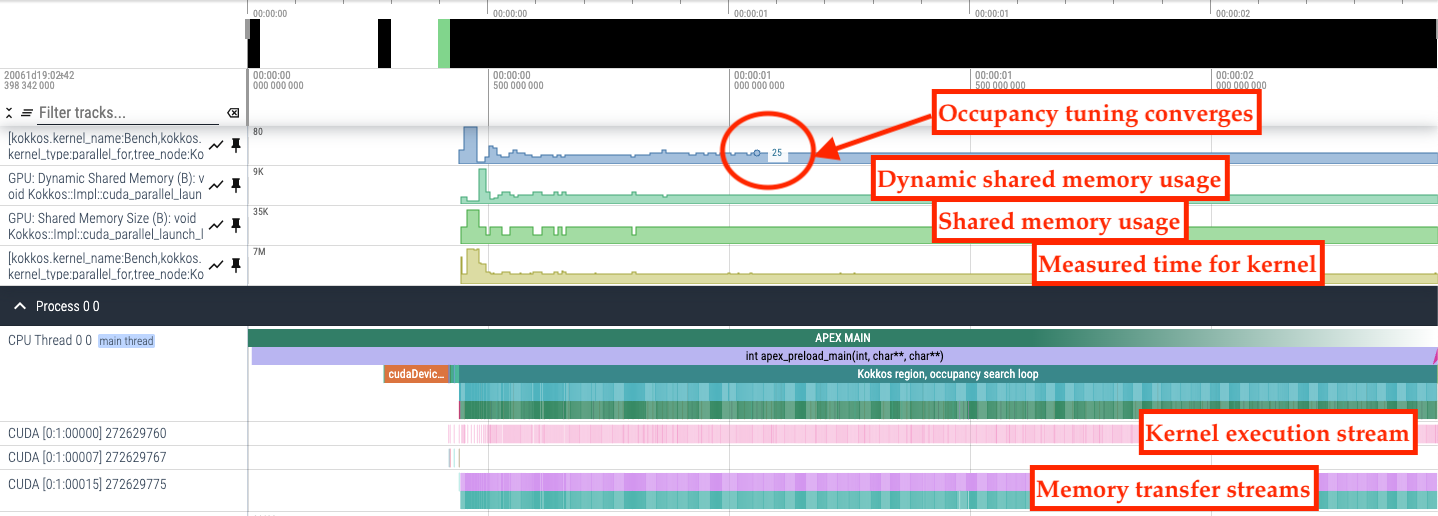
\includegraphics[width=\linewidth]{4_5/tuning/nelder_mead_occupancy_trace.png}
    \end{center}
\end{frame}

\begin{frame}[fragile]{Kokkos Potential Future Tuning Plans (7/7)}
  \begin{itemize}
      \item Simplified/abstracted API for custom tuning in user code (or at least some helper functions)
      \begin{itemize}
        \item \texttt{kokkosp\_declare\_[input,output]\_type} - make it easier to create variables
        \item \texttt{kokkosp\_[begin,end]\_context}
        \item \texttt{kokkosp\_request\_values}
      \end{itemize}
      \item Additional examples, performance studies
      \item Internal tuning for \texttt{RangePolicy}
      \item Internal support/testing for more execution engines (SYCL, OpenMP, OpenMPTarget)
  \end{itemize}
\end{frame}

%==========================================================================


%==========================================================================


% Makefile and CMake support for C++23
% Update minimum compiler versions. (covered in earlier section)

\begin{frame}[fragile]{Build System Updates}
\textbf{C++ Standards Support}
\begin{itemize}
  \item \texttt{CMAKE\_CXX\_STANDARD=23} is supported
  \begin{itemize}
    \item \texttt{KOKKOS\_CXX\_STANDARD} for the Makefile
  \end{itemize}
  \item In CMake Kokkos will default to C++17 if no standard is specified
\end{itemize}
\end{frame}

%==========================================================================

% Let CMake determine OpenMP flags.
% Only add -latomic in generated GNU makefiles when OpenMPTarget backend is enabled

\begin{frame}[fragile]{Build System Updates}
\textbf{OpenMP and OpenMPTarget}
\begin{itemize}
  \item OpenMP flags are now determined by CMake's FindOpenMP
  \item Makefile: \texttt{libatomic} only linked in OpenMPTarget builds
\end{itemize}
\end{frame}

%==========================================================================

% Do not add -cuda to the link line with NVHPC compiler when the CUDA backend is not actually enabled
% Kokkos_ENABLE_CUDA_LAMBDA now ON by default with NVCC
% Fix enabling of relocatable device code when using CUDA as CMake language
% Fix cmake configuration with CUDA 12

\begin{frame}[fragile]{Build System Updates}
\textbf{CUDA}
\begin{itemize}
  \item \texttt{Kokkos\_ENABLE\_CUDA\_LAMBDA} set to \texttt{ON} by default
  \item Fixes to RDC flags when using CMake CUDA language
  \item Fixed CUDA 12 when using \texttt{nvcc\_wrapper} with CMake
  \item Fixes to using NVHPC as a compiler when CUDA is not enabled
\end{itemize}
\end{frame}

%==========================================================================


%==========================================================================

\begin{frame}[fragile]

  {\Huge Potentially Breaking Changes}
  
    \vspace{10pt}

\end{frame}

%==========================================================================

\begin{frame}[fragile]{Breaking Changes 1/1}

\begin{itemize}

\item Dropped \texttt{Array} special treatment in \texttt{View}
  \begin{itemize}
  \item was treated as an extra compile-time dimension in the view
  \item now able to construct unmanaged view of arrays
  \end{itemize}

\item Got rid of \texttt{Experimental::RawMemoryAllocationFailure}
  \begin{itemize}
  \item no known usage
  \item internally catching them and rethrowing regular \texttt{std::runtime} exceptions
  \end{itemize}

\item Bug fix for thread safety can lead to deadlocks if user code violates Kokkos sematics
      (see \textbf{Bug Fixes - Thread Safety} and \textbf{View of Views})

\end{itemize}

\end{frame}


%==========================================================================

\begin{frame}[fragile]

  {\Huge Deprecations}
  
    \vspace{10pt}

\end{frame}

\begin{frame}[fragile]{Deprecations}
\begin{itemize}
\item Deprecated allocation step inside \texttt{deep\_copy(UnorderedMap,UnorderedMap)}
  \begin{itemize}
    \item[] Maps now must have the same capacity to \texttt{deep\_copy}
  \end{itemize}
\item Deprecated implicit conversions of integers to \texttt{ChunkSize}
\begin{itemize}
  \item[] Behavior only introduced in 4.3
\end{itemize}
\item Deprecated implicit conversions to all execution spaces
\end{itemize}

\end{frame}

%==========================================================================

\begin{frame}[fragile]{Deprecate \texttt{Array<...,Proxy>} Argument}
\begin {itemize}
\item Deprecated trailing \texttt{Proxy} template argument in \texttt{Kokkos::Array}
\begin{code}
// DEPRECATED
// template <typename T = void,
//           size_t N = KOKKOS_INVALID_INDEX,
//           typename Proxy = void>
template <typename T, size_t N>
struct Array { /* ... */ };
\end{code}
  \begin{itemize}
    \item Deprecates \textit{non-owning, dynamically sized} \texttt{contiguous/strided} functionality
    \item More in line with (always) \textit{owning} \& \textit{statically sized} \texttt{std::array}
  \end{itemize}
\end{itemize}
\end{frame}

%==========================================================================

\begin{frame}[fragile]{Deprecate \texttt{is\_layouttiled}}
\begin {itemize}
\item Removed \texttt{Kokkos::Experimental::LayoutTiled} class template
  \begin{itemize}
  \item Never useable
  \end{itemize}
\item Deprecated \texttt{is\_layouttiled} trait
  \begin{itemize}
  \item Not useful, but no rush to remove it
  \end{itemize}
\item Deprecated \texttt{Kokkos::layout\_iterate\_type\_selector}
  \begin{itemize}
  \item Not useful outside of Kokkos implementation
  \end{itemize}
\end{itemize}
\end{frame}

%==========================================================================
\begin{frame}[fragile]{Deprecate \texttt{pair<T,void>}}
\begin {itemize}
\item Deprecated specialization of \texttt{Kokkos::pair} for a single element
\begin{code}
// DEPRECATED
// template <typename T>
// struct pair<T, void> { /* ... */ };
\end{code}
  \begin{itemize}
  \item Never supported in \texttt{std::pair}
  \item Never documented
  \item Never tested
  \item No known usage
  \end{itemize}
\end{itemize}
\end{frame}

%==========================================================================

%==========================================================================

\begin{frame}[fragile]

  {\Huge Bug Fixes}

  \vspace{10pt}

\end{frame}

%==========================================================================

% Examples

% note: always keep the [fragile] for your frames!

%\begin{frame}[fragile]{Example list}
%  \begin{itemize}
%      \item Item 1
%      \item Item 2 with some \texttt{code}
%      \begin{itemize}
%        \item Sub-item 2.1
%        \item Sub-item 2.2
%      \end{itemize}
%  \end{itemize}
%\end{frame}

%\begin{frame}[fragile]{Example code}
%    \begin{code}[keywords={std}]
%        #include <iostream>
%        
%        int main() {
%            std::cout << "hello world\n";
%        }
%    \end{code}
%\end{frame}

%\begin{frame}[fragile]{Example table}
%    \begin{center}
%        \begin{tabular}{l|l}
%            a & b \\\hline
%            c & d
%        \end{tabular}
%    \end{center}
%\end{frame}

%==========================================================================

\begin{frame}[fragile]{General Bug Fixes}
    \begin{itemize}
      \item Fix a memory leak from an early exit when using \texttt{--kokkos-tools-help} % 8074
      \item Add missing fences for async Random init with unified memory % 8105
      \item More robust checks on subview constructor % #8210
        \begin{code}[keywords={std}]
View<T**, LayoutLeft> a(N,N);

// Previously allowed, but data should have strided access.
View<T*, LayoutLeft> sub_a(a, 1, ALL); // Runtime Error
        \end{code}

    \end{itemize}
\end{frame}

%==========================================================================

\begin{frame}[fragile]{General Bug Fixes}
  \begin{itemize}
    \item SIMD:
    \begin{itemize}
      \item Fix compile errors with \texttt{Kokkos\_ARCH\_NATVE=ON} % 7912
      \item Fix fallback simd masked reductions using incorrect identity elements % 8115
    \end{itemize}
    \item Compilers:
    \begin{itemize}
      \item Apply a workaround for a segfault issue in \texttt{SharedAllocationTracker} with gcc 12.2, 12.3 and 12.4 % 8223
      \item Fix compiling with C++23 supported compilers that provide an mdspan implementation % #8234
    \end{itemize}
  \end{itemize}
\end{frame}

%==========================================================================

\begin{frame}[fragile]{Backend Bug Fixes}
    \begin{itemize}
        \item HPX: fix to constrain hpx\_thread\_buffer size used with TeamPolicy setup % #8147
        \item HIP and SYCL:
        \begin{itemize}
          \item A \texttt{MDRangePolicy} of rank 4 or more would be incorrectly iterated, leading to some iterations being evaluated more than once for large enough loops % 7880
        \end{itemize}
        \item HIP:
        \begin{itemize}
          \item \texttt{ConstantMemory} launch mechanism would sporadically fail due to \texttt{hipEventSynchronize} error % 8094
          \item Fix launch of intermediate size functors in graph % #8188
        \end{itemize}
        \item Serial: memory leak in internal instance data % 8042
        \item OpenMP Target and OpenACC: An out-of-bounds access would occur in \texttt{Random\_UniqueIndex} under certain circumstances % 8077
    \end{itemize}
\end{frame}





%==========================================================================

\begin{frame}[fragile]

  \vspace{10pt}

  \textbf{How to Get Your Fixes and Features into Kokkos}
  \newline
  \begin{itemize}
    \item Fork the Kokkos repo (\url{https://github.com/kokkos/kokkos})
    \item Make topic branch from \textit{develop} for your code
    \item Add tests for your code
    \item Create a Pull Request (PR) on the main project \textit{develop}
    \item Update the documentation (\url{https://github.com/kokkos/kokkos-core-wiki}) if your code changes the API
    \item Get in touch if you have any question (\url{https://kokkosteam.slack.com})
  \end{itemize}

\end{frame}

%==========================================================================

\end{document}
